\begin{figure}[t!]
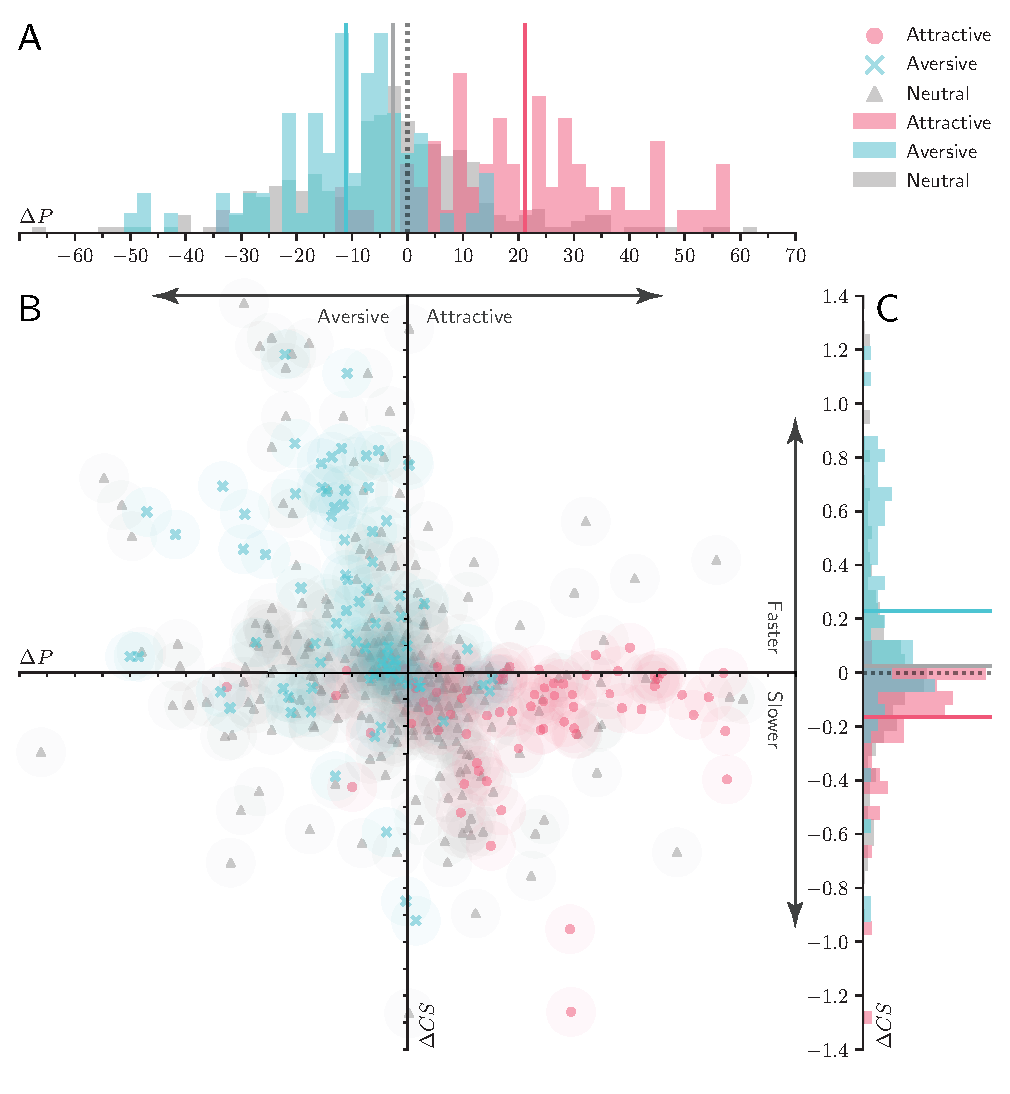
\includegraphics[width=\linewidth]{Figures/images/4.eps}
 \captionof{figure}{\textbf{Larval stimulus preference is correlated to concentration-dependent movement speed.} A: Larval preference (${\Delta}$P) significantly correlates with Concentration-dependent Speed (${\Delta}$CS). Results from all experiments are shown grouped into three categories: attractive (pink: food, food extract, and yeast RNA in starved larvae), aversive (blue: quinine), and neutral (grey: water, indole, o-cresol in fed and starved larvae; food, food extract, and yeast RNA in fed larvae). B: Normalized frequency histograms of ${\Delta}$P. Mean response to aversive, neutral, and appetitive cues are visualized as solid vertical lines in the corresponding color. A dotted black line at zero indicates the expected outcome if the added stimulus had no effect on larval behavior. C: As in B, except for normalized frequency histograms of larval ${\Delta}$CS.
 }
 \label{fig:fig1}
\end{figure}